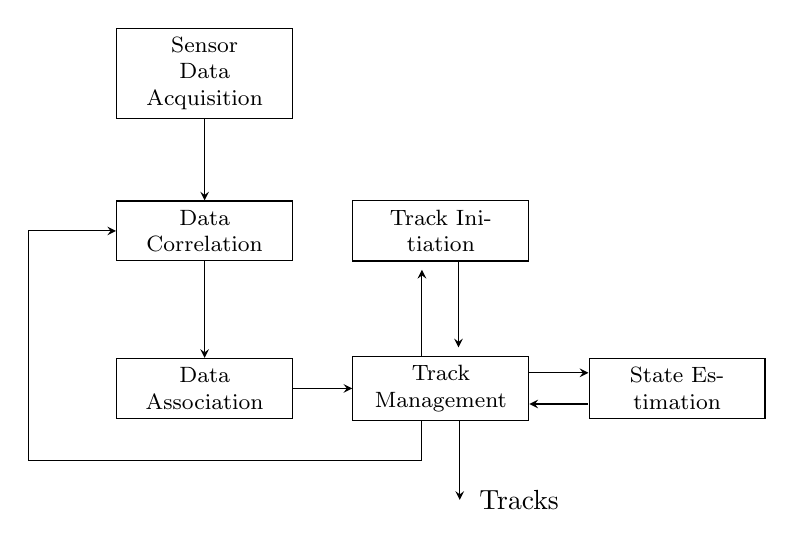
\begin{tikzpicture}[xscale=1,yscale=1,
	square/.style={rectangle, draw=black, text width=20mm, align=center, font=\footnotesize},
	label/.style={text width=5mm, align=center},
	node distance= 2cm, >=stealth]
	
	%Nodes
	\node[square]	(sda)	at (0,0) {Sensor\\Data\\Acquisition};
	\node[square]	(dc)	[below of=sda] {Data\\Correlation};
	\node[square]	(da)	[below of=dc] {Data\\Association};
	\node[square, xshift=1cm]	(ti)	[right of=dc] {Track Initiation};
	\node[square]	(tm)	[below of=ti] {Track\\Management};
	\node[square, xshift=1cm]	(se)	[right of=tm] {State Estimation};
	
	%Lines
	\draw[black, ->] (sda) -- (dc);
	\draw[black, ->] (dc) -- (da);
	\draw[black, ->] (da) -- (tm);
	\draw[black, ->] (ti.300) -- ++(0,-1.09);
	\draw[black, ->] (tm.120) -- ++(0,1.09);
	\draw[black, ->] (tm.10) -- ++(0.75,0);
	\draw[black, <-] (tm.350) -- ++(0.75,0);
	\draw[black, ->] (tm.240) -- ++(0,-0.5) -- ++(-5,0) |- (dc.west);
	\draw[black, ->] (tm.300) -- ++(0,-1) node[label, xshift=5mm] {Tracks};
\end{tikzpicture}